
\documentclass{beamer}
%
% Choose how your presentation looks.
%
% For more themes, color themes and font themes, see:
% http://deic.uab.es/~iblanes/beamer_gallery/index_by_theme.html
%
\mode<presentation>
{
	\usetheme{default}      % or try Darmstadt, Madrid, Warsaw, ...
	\usecolortheme{default} % or try albatross, beaver, crane, ...
	\usefonttheme{default}  % or try serif, structurebold, ...
	\setbeamertemplate{navigation symbols}{}
	\setbeamertemplate{caption}[numbered]
} 

\usepackage[english]{babel}
\usepackage[utf8]{inputenc}
\usepackage[T1]{fontenc}
\usepackage{graphicx}
\usepackage{subfigure}
\usepackage[font=small,labelfont=bf]{caption}


\title[Your Short Title]{Progresses in data analysis an ABM}
\date{31/03/20}

\begin{document}
	
	\begin{frame}
	\titlepage
\end{frame}

% Uncomment these lines for an automatically generated outline.
%\begin{frame}{Outline}
%  \tableofcontents
%\end{frame}

\begin{frame}{Data Analysis}
\begin{itemize}
	\item The Taxi Time distributions for different companies are different.
\end{itemize}
 \begin{minipage}{\textwidth}
	\begin{minipage}[b]{0.49\textwidth}
		\centering
		\includegraphics[scale=0.26]{taxiTimeCompanies.png}

	\end{minipage}
	\hfill
	\begin{minipage}[b]{0.3\linewidth}
		\centering
		\tiny
		\begin{tabular}{p{1cm}p{2cm}}\hline
			Company & Avarage Taxi Time \\ \hline
			AFR & 433 s \\
			EZY & 460 s \\
			FDX & 548 s \\ \hline
		\end{tabular}
\bigskip
\bigskip
\bigskip
\bigskip
\bigskip
\bigskip
\bigskip

	\end{minipage}
\end{minipage}
\end{frame}


\begin{frame}{Data Analysis}

	 Is taxi time dependant on the company or only on the hour of take off and landing?




\begin{itemize}
	\item We sampled Air France flights (48,3\% of total flights) based on the time distribution of movements for other companies, i.e. Easy Jet (6,52\%) and FedEx (2,25\%).
\end{itemize}


\end{frame}


\begin{frame}{Results}
\begin{itemize}
	\item The different movement's time distribution don't explain the variation in taxi time.
\end{itemize}
\begin{minipage}{\textwidth}
	\begin{minipage}[b]{0.49\textwidth}
		\centering
		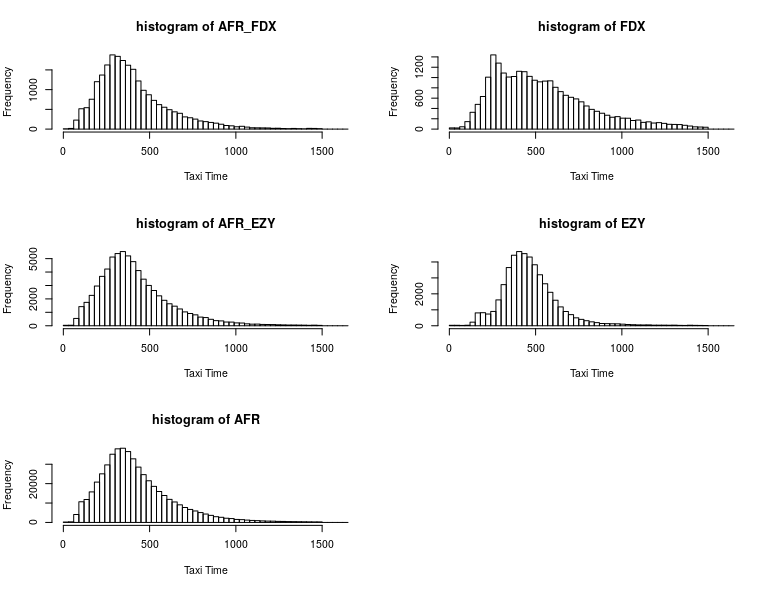
\includegraphics[scale=0.35]{taxi_time_sample_AFR.png}
	\end{minipage}
	\hfill
	\begin{minipage}[b]{0.3\linewidth}
		\centering
		\tiny
		\begin{tabular}{p{1.1cm}p{2cm}}\hline
			Company & Avarage Taxi Time \\ \hline
			AFR & 433 s \\
			AFR-EZY & 429 s\\
			EZY & 460 s \\
			AFR-FDX & 432 s\\
			FDX & 548 s \\ \hline
		\end{tabular}

		\bigskip
		\bigskip
		\bigskip
		\bigskip
		\bigskip
		\bigskip
		
	\end{minipage}
\end{minipage}
\end{frame}


\begin{frame}{ABM Model: LIFO vs FIFO policy}
We asked ourselves about how different policies in the outgoing traffic could change the waiting time at the runway. We experimented the first-in-first-out and last-in-first-out policies to see how the waiting time distribution changed.

		\centering
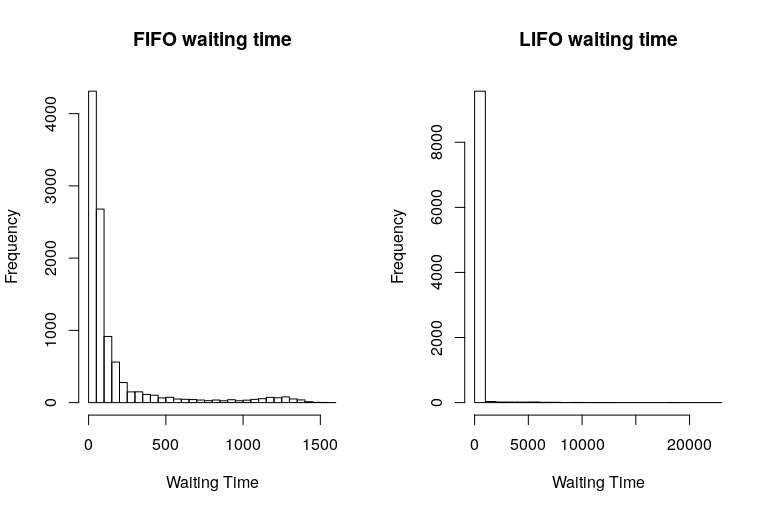
\includegraphics[scale=0.4]{FIFO-LIFO.png}


\end{frame}

\begin{frame}{ABM Model: LIFO vs FIFO policy}

\begin{minipage}{\textwidth}
	\begin{minipage}[b]{0.49\textwidth}
		\centering
		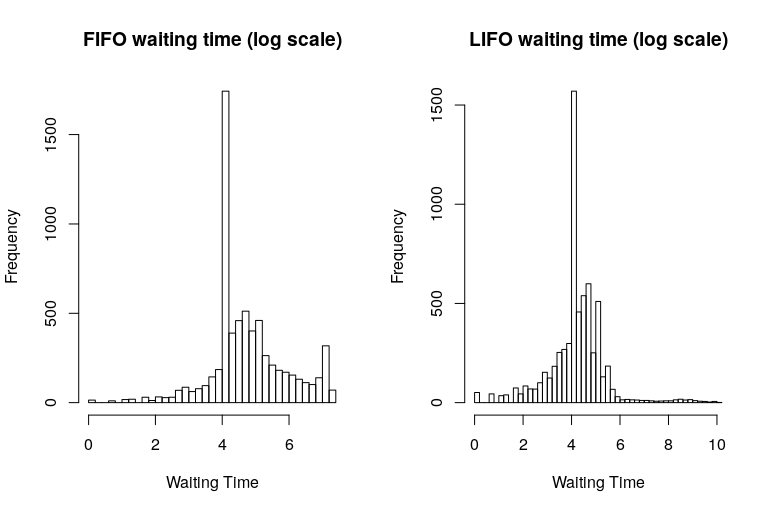
\includegraphics[scale=0.35]{FIFO-LIFOlog.png}
	\end{minipage}
	\hfill
	\begin{minipage}[b]{0.3\linewidth}
		\centering
		\tiny
		\begin{tabular}{p{1.1cm}p{1.1cm}}\hline
			\smallskip Policy & Avarage Waiting Time \smallskip \\ \hline
			\smallskip FIFO & \smallskip 149 s \\
			LIFO \smallskip & 147 s\\ \hline
		\end{tabular}
		
		\bigskip
		\bigskip
		\bigskip
		\bigskip
		
	\end{minipage}
\end{minipage}
We see a peak in correspondance to the waiting time = 60 because in the simulation, when the plane arrives at the runway, it has a certain probability to have to stop and wait 60 seconds for another plane to land.

\end{frame}
\end{document}

